\documentclass[conference]{acmsiggraph}

\TOGonlineid{45678}
\TOGvolume{0}
\TOGnumber{0}
\TOGarticleDOI{1111111.2222222}
\TOGprojectURL{}
\TOGvideoURL{}
\TOGdataURL{}
\TOGcodeURL{}

\title{Painterly Rendering for WebGL}

\author{Andy Hanson\thanks{email: hansoa2@rpi.edu}\\
        Scott Todd\thanks{email: todds@rpi.edu}}
\pdfauthor{Robert A. Smith}

\keywords{radiosity, global illumination, constant time}

\begin{document}

\teaser{
  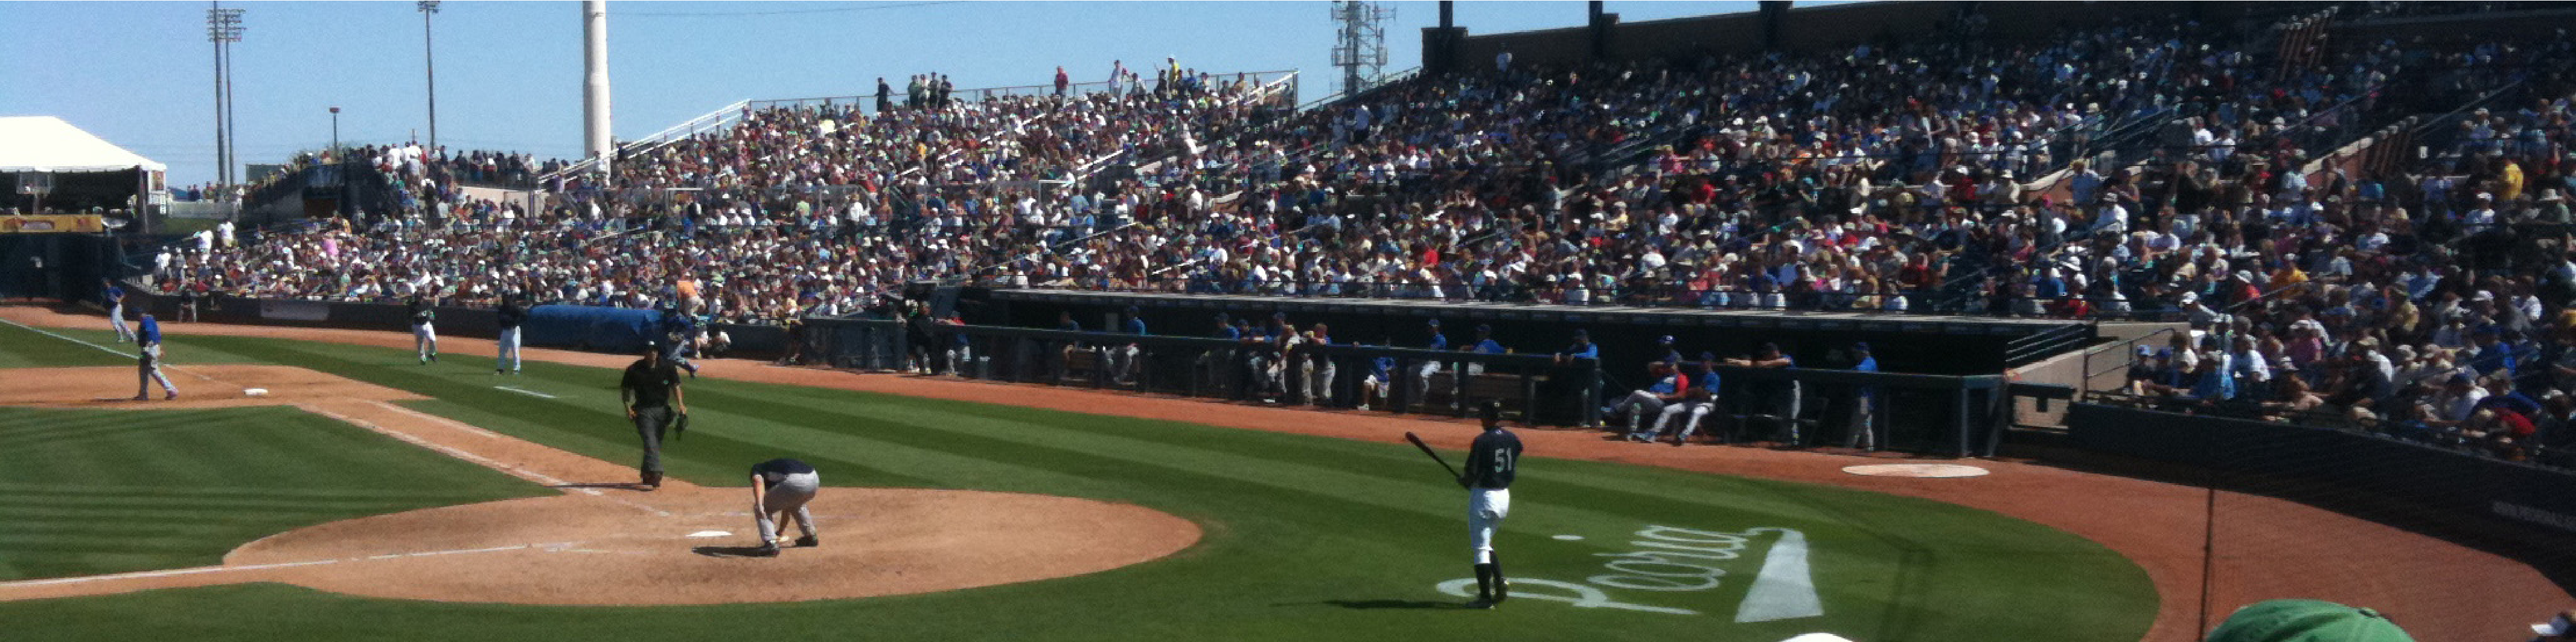
\includegraphics[height=1.5in]{images/sampleteaser}
  \caption{Spring Training 2009, Peoria, AZ.}
}

\maketitle

\begin{abstract}

TODO.

\end{abstract}

%%% The ``CRCatlist'' environment defines one or more ACM ``Computing Review''
%%% (or ``CR'') categories, used for indexing your work. For more information
%%% on CR categories, please see http://www.acm.org/class/1998.

% \begin{CRcatlist}
%   \CRcat{I.3.3}{Computer Graphics}{Three-Dimensional Graphics and Realism}{Display Algorithms}
%   \CRcat{I.3.7}{Computer Graphics}{Three-Dimensional Graphics and Realism}{Radiosity};
% \end{CRcatlist}

\keywordlist

%% Use this only if you're preparing a technical paper to be published in the
%% ACM 'Transactions on Graphics' journal.

\TOGlinkslist

%% Required for all content.

\copyrightspace

\section{Introduction}

TODO.

(Link to GitHub and hosted url)

\subsection{Related Work}

TODO \cite{Meier:1996:PRA:237170.237288}.

\section{Painterly Rendering System}

\subsection{Algorithm Overview}

Our system takes as input a set of three.js geometries and a list of rendering
parameters for each geometry, as well as a list of three.js directional lights.
It outputs to a three.js WebGL renderer in any supporting browser.

TODO.

\begin{figure}[ht]
  \centering
  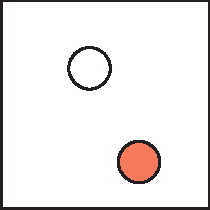
\includegraphics[width=1.5in]{images/samplefigure}
  \caption{Sample illustration.}
\end{figure}

\subsection{Stroke Selection}

TODO.

\section{Stroke Rendering}

We represent each brush stroke as a particle within a particle system that is
maintained by three.js. We provide a vertex shader and a fragment shader for
three.js to use in rendering the particle system. Each layer of brush strokes
on each object in the scene has its own particle system.

\subsection{zQuality}

\begin{figure*}[ht] % figure* allows for this to span the full page width
  \centering
  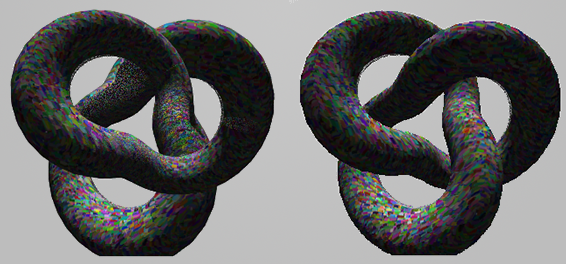
\includegraphics[width=6.0in]{images/torus_depth_test_demo}
  \caption{The image on the right discards fragments whose depth values differ
           from the value stored in the depth buffer texture while the image on
           the left does not. Note the intersections and other artifacts on the
           left.}
\end{figure*}

We found that three.js could sort particles by depth for rendering, but this
was too slow for our application and the number of particles we were using.
Blending within the shaders was also unsuccessful.

We use a two-pass rendering approach to perform z-culling. First, we render
only the original geometry into a floating point depth buffer texture. Then, we
pass that texture into our brush stroke shaders and use that information to
choose which strokes to render.

In the first iteration of our algorithm, we discarded fragments whose depth
values differ from the value stored in the depth buffer at that position. This
method performs a sharp cutoff around the silhouette of each object, so it
conflicted with the painterly rendering focus of our project.

We refined this approach by expanding the silhouette of each object in the
scene and fading strokes in based on the difference between their depth and the
depth in the depth buffer texture. We expanded the silhouette of each object by
pushing each vertex of their geometries by a factor of the normal at that
vertex.

\subsection{Gradient Estimation}

\begin{figure*}[ht]
  \centering
  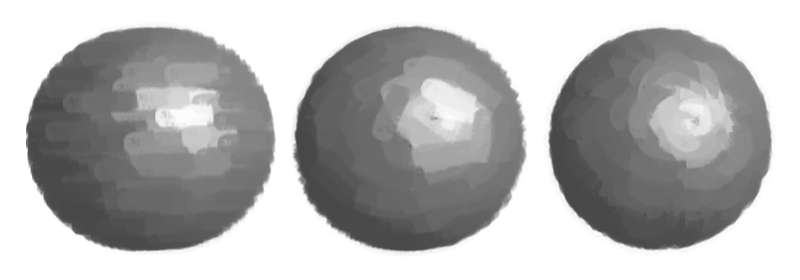
\includegraphics[width=6.0in]{images/sphere_rotation_curve}
  \caption{From left to right: no orientation or curvature, orientation with
           no curvature, orientation and exaggerated curvature (2.0).}
\end{figure*}

TODO.

\subsection{Layering}

TODO.

\subsection{Parameters List}

TODO.

\section{Results}

TODO.

\begin{figure}[ht]
  \centering
  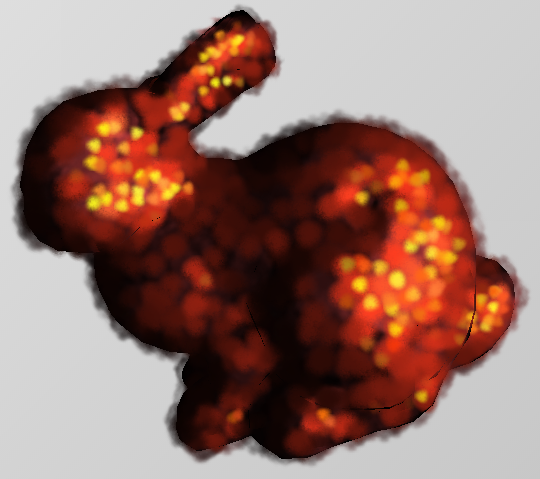
\includegraphics[width=3.3in]{images/bunny_with_fade_in}
  \caption{The Stanford bunny rendered using three layers of brush strokes.
           The topmost layer uses a minimum specular cutoff of 0.95 and a
           specular fade-in of 0.63.}
\end{figure}

\begin{figure}[ht]
  \centering
  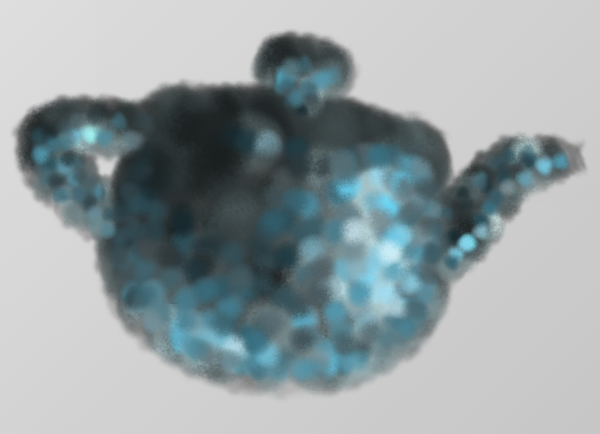
\includegraphics[width=3.3in]{images/teapot_with_background}
  \caption{The Utah teapot rendered using three layers of brush strokes.
           The topmost layer uses a specular fade-in of 0.03.}
\end{figure}

\section{Limitations}

TODO.

\section{Future Work}

TODO.

\section{Conclusion}

TODO.

\section*{Acknowledgements}

(TODO) Three.js

\bibliographystyle{acmsiggraph}
\bibliography{painterly_rendering}
\end{document}
